\documentclass[a4paper,10pt]{article}

\usepackage{chin-report}

\begin{document}
\fontfamily{lmss}\selectfont

{
	\small
    \hspace*{-0.3cm}  
    \begin{tabularx}{168mm}{ l X|X r }
        %\hline
        \multirow{7}{*}{
\includegraphics[width=9.8cm]{unilogo}} & & & BIO-4371 \\
	    & & & \textcolor{UT_RED}{\textbf{Structure-Based Drug Design}}  \\ [2pt]
        & & & Summer Semester 2025 \\
        & & & \\
        & & & Institute for Bioinformatics \\
        & & & and Medical Informatics \\
        %\hline
    \end{tabularx}
}


\begin{huge}
	\vspace{1cm}
	\textbf{SBDD Project}
\end{huge} \\

Authors: Sarah Hüwels, Mattes Warning, Mona Scheurenbrand 

\begin{large}
	\vspace{0.5cm}
	\textbf{Introduction}
\end{large}	\\ [1mm]

Predicting the position and orientation of a ligand when bound to a receptor is referred to as \textbf{protein-ligand docking}.
We investigate the quality of the widely used docking tool \textit{Autodock vina} \cite{eberhardt2021autodock} with respect to two tasks: 1) Predicting the binding pose of a known ligand and
2) performing virtual screening (VS). Pose predicting quality is quantified by the atom root-mean-square deviation (RMSD) between docked and crystallographic poses, accepting $\leq$ 2.0 Å as successful.
Virtual screening performance is measured by the area under the receiver-operating characteristics curve (ROC-AUC) when docking 40 know ligands and 1200 decoys.

To benchmark Vina across different biological contexts, we selected four targets: 1A4G, 1OUK, 1E3G, and 1CX2. Please refer to the individual sections for more detailed descriptions of these targets.

\begin{large}
	\vspace{0.5cm}
	\textbf{Materials and Methods}
\end{large}	\\ [1mm]

\textbf{Protein-ligand docking}

\textit{Target: 1A4G}

We started the ligand and receptor preparation by removing all solvent molecules using Pymol. 
For ligand preparation, we inspected the ligands and used the chains that are bound to the target. For 1A4G we used a ZMR residue in chain A. We saved the ligand molecule as PDB file.
For the receptor preparation, we selected everything, except ZMR residues, and saved the resulting receptor molecule to a PDB file.

Next, PDB files were converted into .pdbqt format using Open Babel to support active torsion information and charges for atoms. 

We used the Vina force field (scoring function) to do docking and a random seed = 12345 to ensure reproducible results. To choose the box center and box size for docking, we extracted the ligand bounding box min and max coordinates in Pymol with this command: \textit{get$\_$extent ligand$\_$name}. Those are in the format (minX, minY, minZ) and (maxX, maxY, maxZ). The centers for the three coordinates x, y, z are then calculated, by taking the average of the min and max coordinates. The box size is calculated by (max-min)+4, where 4 is the margin in Å. The resulting values are then used for the parameters \textit{center$\_$x}, \textit{center$\_$y}, \textit{center$\_$z}, \textit{size$\_$x}, \textit{size$\_$y}, and \textit{size$\_$z}.

\begin{table}[h!]
\centering
\caption{Ligand bounding box min and max coordinates}
\label{tab:box}
\begin{tabular}{|c|c|c|c|c|c|c|}
\hline
\textbf{Ligand (Receptor)} & \textbf{minX} & \textbf{minY} & \textbf{minZ} & \textbf{maxX} & \textbf{maxY} & \textbf{maxZ} \\
\hline
ZMR (1A4G) & -7.638 & 53.013 & -12.316&1.912 &59.198 &-4.813 \\
084 (1OUK) &37.814  &26.313  &28.994 &50.830 &38.599 &34.278 \\
R18 (1E3G) & -3.502  & 26.212  &2.412 &3.375 &35.553 & 6.189\\
S58 (1CX2) & 18.483  & 18.488  & 10.836 & 29.412 & 24.676 & 20.036\\
\hline
\end{tabular}
\end{table}


To assess the prediction quality, we compared the predicted pose with the experimentally observed pose of the original PDB file by calculating root-mean-square deviation (RMSD). We assumed a docking pose with RMSD < 2.0 Å to be correct.

\textit{Target: 1OUK-p38 alpha}

1OUK-p38 alpha is  a human p38 alpha MAP kinase. This protein is a target for the treatment of inflammation and is therefore interesting for drug development. Molecules, that bind to this molecule, could act as inhibiors and can suppress its kinase activity. This would reduce the expression of downstream inflammatory genes. \cite{1OUK}

During the ligand and receptor preparation the residue 084 was identified as a suitable ligand and written into a .pdb file. The molecule including everything except the residue 084 was used as receptor and also written to a .pdb file. 

The bounding box coordinates are given in Table \ref{tab:box} and VS is done analog to the 1A4G target.

\textit{Target: 1E3G}
..


\textit{Target: 1CX2 Cox2}

1CX2 is the PDB identifier for the crystal structure of cyclooxygenase-2 (COX-2). COX-2 is an enzyme that plays a key role in the inflammatory response by catalyzing the conversion of arachidonic acid to prostaglandins \cite{1CX2}. In contrast to COX-1, which is a constitutively expressed isoform of COX-2, COX-2 is inducible and is often overexpressed at sites of inflammation \cite{1CX2_2}. This makes it an interesting target for anti-inflammatory drug development. For this, protein-ligand docking and virtual screening are helpful to identify molecules that can bind to its active site. 

For 1CX2, the ligand S58 was identified and the receptor and ligand were separately stored in a .pdb file. See Table \ref{tab:box} for bounding box coordinates used for subsequent box center computations for docking. VS was conducted as described for 1A4G.





\textbf{Virtual Screening}

\textit{Target: 1A4G}

For VS, docking of several compounds against the prepared receptor was performed. Compounds were split into known true ligands (n = 40) and known non-binders (decoys, n = 1200) and the binding affinity of the best prediction of every docked compound together with the label were merged into a final result list for ranking. The box center and box size was calculated as described during protein-ligand-docking.
VS quality assessment for each receptor was performed using the receiver operating characteristic (ROC) curve and calculating the area under the curve (AUC).


\begin{large}
	\vspace{0.5cm}
	\textbf{Results}
\end{large}	\\ [1mm]

\textbf{Protein-ligand docking}

Protein-ligand docking was performed using the prepared receptor 1A4G - \textit{Neuraminidase} - and the prepared ligand \textit{ZMR}. The RMSD between the predicted pose and the experimentally observed pose was 0.1 Å. Thus, this predicted docking pose can be considered correct. Further, the RMSD between each possible pose and the observed pose was calculated (Table \ref{tab:rmsd}). All poses have a RMSD score below 2Å and can be considered correct. The first pose is the best pose compared to the remaining poses, since it has the lowest RMSD value.


\begin{table}[h!]
\centering
\caption{RMSD values of docking poses}
\label{tab:rmsd}
\begin{tabular}{|c|c|c|}
\hline
\textbf{Pose} & \textbf{RMSD [\AA]} & \textbf{Predicted Binding Affinity [kcal/mol]} \\
\hline
1 & 0.10 & -8.005\\
2 & 0.20 & -7.788\\
3 & 0.35 & -7.344\\
4 & 0.96 & -7.063\\
5 & 0.85 & -6.811\\
6 & 0.29 & -6.784 \\
7 & 1.04 & -6.719 \\
8 & 0.25 & -6.672\\
9 & 1.17 & -6.555 \\
\hline
\end{tabular}
\end{table}


\textbf{Virtual Screening}
Virtual Screening was assessed by generating a ROC curve using the predicted binding affinity score and the true labels for true ligands and decoys for each receptor. The Area under the curve (AUC) value describes, how well the screening can distinguish between true positives, so active compounds, and false positives, inactive compounds. 


\begin{figure}[h!]
  \centering

  \begin{subfigure}{0.45\linewidth}
    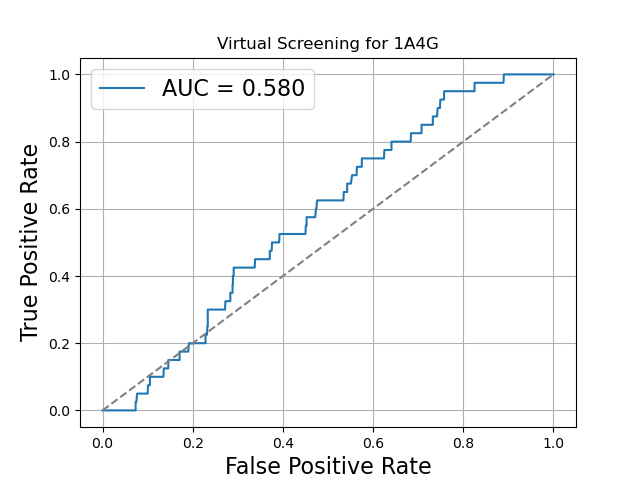
\includegraphics[width=\linewidth]{figures/ROC.png}
    \caption{1A4G}
    \label{fig:a}
  \end{subfigure}
  \hfill
  \begin{subfigure}{0.45\linewidth}
    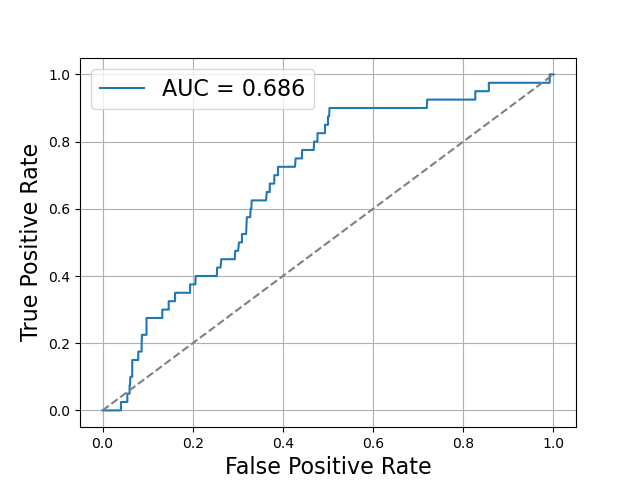
\includegraphics[width=\linewidth]{figures/ROC-1OUK.png}
    \caption{1OUK}
    \label{fig:b}
  \end{subfigure}

  \vspace{1em}

  \begin{subfigure}{0.45\linewidth}
    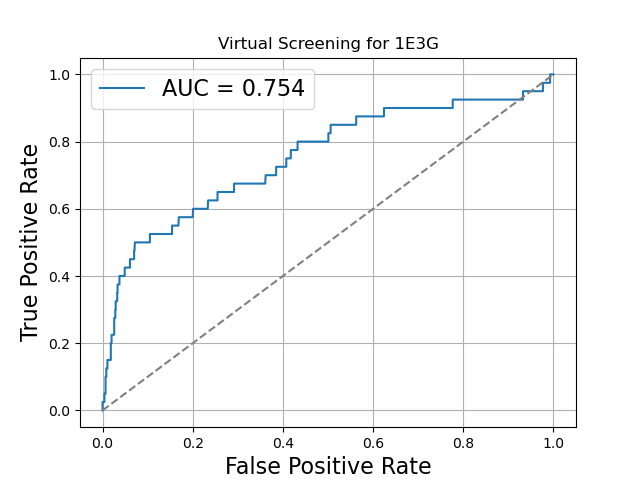
\includegraphics[width=\linewidth]{figures/ROC_1E3G.png}
    \caption{1E3G}
    \label{fig:c}
  \end{subfigure}
  \hfill
  \begin{subfigure}{0.45\linewidth}
    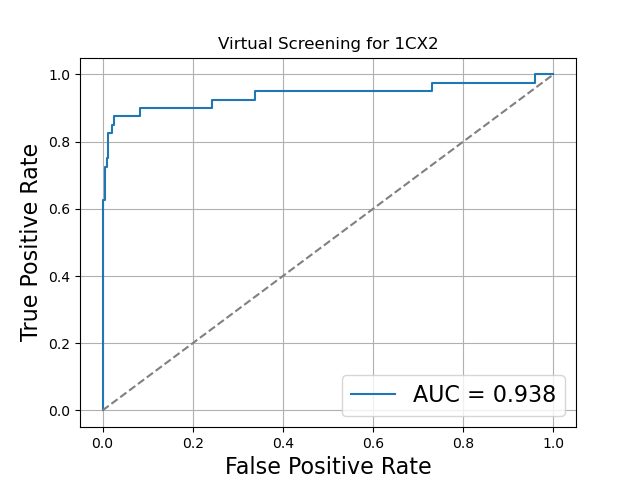
\includegraphics[width=\linewidth]{figures/ROC_1CX2.png}
    \caption{1CX2}
    \label{fig:d}
  \end{subfigure}

  \caption{ROC curves for VS assessment}
  \label{fig:ROCs}
\end{figure}



\textit{Target: 1A4G} 

For the target Neuriaminidase we get an AUC of 0.580 (see Figure \ref{fig:a}), which suggests that the performance is slightly better than random guessing. 



\textit{Target: 1OUK-p38 alpha}


For the target 1OUK-p38 alpha we get a AUC of 0.686 (see Figure \ref{fig:b}), which suggests that the performance is better than random guessing, but there is still room for improvement.

\textit{Target: 1E3G}

(see Figure \ref{fig:c})
..

\textit{Target: 1CX2}

With an AUC of 0.938 (see Figure \ref{fig:d}), virtual screening assessment for 1CX2 achieved the highest performance among all targets. This indicates a strong ability of the screening tool to distinguish between active and inactive compounds for this protein.




\begin{large}
	\vspace{0.5cm}
	\textbf{Discussion}
\end{large}	\\ [1mm]

The pose-prediction quality of the docking tool for the target 1A4G and the ligand ZMR produced a good result. The pose ranked highest by docking score, i.e., predicted binding affinity, was also  the one with the best RMSD and thus closest to the experimental pose. 

In the Virtual Screening conducted on the four targets, the discriminatory power of the screening was not ideal for the targets 1A4G and 1OUK. For target 1E3G, the screening produced an acceptable AUC value and for the target 1CX2 it yielded a high AUC value, indicating good discriminative power. These results show, that the same scoring function, in our case the vina scoring function, performs very differently across all targets. There is not one scoring function that performs optimal across all targets. To improve the screening performance for 1A4G and 1OUK, alternative scoring functions should be considered for docking.




\textbf{Additional Targets}

Mona Scheurenbrand worked on the target 1cx2-cox2, Mattes Warning worked on 1e3g-ar, and Sarah Hüwels worked on 1ouk$\_$p38-alpha.

\bibliographystyle{plain}
\bibliography{references}

\end{document}

